\chapter{Feature Modelling}
\label{ch:feature modelling}

% 
% In Software Product Lines (SPL)~\cite{PohlBL05}, features are
% associated to software artifacts. Such artifacts are then compiled together
% into executable software products.

% The set of products is represented by a feature
% model~\cite{batory-challenges-2006,KangCHNP90} describing the valid combinations
% of features, such as the feature diagram depicted in
% Fig.~\ref{fig:feature diagram}. Features are associated to software
% artifacts used to build software products from valid selections of features.

% The ABS suite supports SPLE using a range of language constructs and tools.
% First \emph{feature models} can be specified using a textual notation that is
% closely related to feature diagrams. Typically, the developer then specifies a
% \emph{product selection}, which is the set of products that are of particular
% interest to the project. In a product selection, each product is given as an
% enumeration of features and assigned a name for easier reference. The actual
% code that represents the behaviour for each feature is encapsulated in
% \emph{delta modules}, and features are associated to delta modules through
% \emph{configuration} directives.

ABS provides language constructs and tools for modelling variable systems
following Software Product Line (SPL)~\cite{PohlBL05} engineering practices. The
\emph{Micro Textual Variability Language} \muTVL~\cite{clarke-variability-2011}
is the part of ABS used to model all products of an SPL by using features and
feature attributes. A \emph{Product Selection} identifies individual products
that are of particular interest to the project. Section~\ref{sec:feature model}
covers feature modelling with \muTVL and Section~\ref{sec:product selection}
describes how to specify product selections.


% \emph{Delta modules} are reusable units of ABS code which can be applied
% incrementally to an ABS program to adapt its behaviour to conform to a
% particular product. Finally, the \emph{Configuration} associates features to
% delta modules, enabling us to generate the ABS source code for individual
% products simply by naming a product. The Core ABS language (cf.
% Section~\ref{sec:coreabs}) enriched with the above extensions is called
% \emph{Full ABS}.
% 
% Fig.~\ref{fig:delta application} depicts the main steps required to build a
% software product using ABS. The developer first selects the desired features.
% % that will guide the compilation of the final software product, in accordance
% % to the feature model.
% This selection is then used to chose the relevant delta modules. Each of these
% delta modules is applied to a core program in turn. The application of all
% relevant delta modules results in the desired software product.
% 
% The remainder of this section details the ABS language constructs used for
% modelling software product lines. Section~\ref{sec:feature model} introduces
% features models and describes how to select valid products. The delta modelling
% approach is described in Section~\ref{sec:delta}, and the connection between
% features and deltas is made in Section~\ref{sec:spl configuration}. We exemplify
% the approach, using our case-study, in Section~\ref{sec:product generation}.
% Finally, we describe our platform and deployment model in
% Section~\ref{sec:platformvar}. A complete reference of ABS, including the
% constructs for modelling variability, can be found
% in~\cite{ABSRef-2011,clarke-variability-2011}.



\section{Feature Model}
\label{sec:feature model}

As part of the requirements engineering process, software variability is
commonly expressed using \emph{features}. Features are organised in a
\emph{feature model}~\cite{Batory:2006,KangCHNP90}, which is
essentially a set of logical constraints expressing the dependencies between
features. Thus the feature model defines a set of legal feature combinations.
These represent the set of valid software products that can be built from the
given features.

\subsection{Syntax}
\label{sec:mutvl-syntax}

The grammar of \muTVL is given in Figure~\ref{fig:mutvl grammar}. Assume the
presence of two global sets: \fid of feature names and \aid of attribute names.
Names in \fid follow type identifier syntax, while names in \aid follow
identifier syntax (cf. Chapter~\ref{ch:lexical structure}).


\begin{figure}[htp]
	\centering

      \begin{tabular}{rcl}
        \NT{Model}
        \concrDefn{
          \MANY{(\TR{root} \NT{FeatureDecl})} \MANY{\NT{FeatureExtension}}}
        \medskip
        \\
        \NT{FeatureDecl}
          \concrDefn{
          %\fid
          %\concrCont{
          %$|$
            \fid \OPTG{\TRS{\{} \OPT{\NT{Group}} \MANY{\NT{AttributeDecl}}
            \MANY{\NT{Constraint}} \TRS{\}}}}
        \\
        \NT{FeatureExtension}
        \concrDefn{
          \TR{extension} \fid \TRS{\{} \MANY{\NT{AttributeDecl}}
          \MANY{\NT{Constraint}}\TRS{\}}}
        \medskip
        \\
        \NT{Group}
              \concrDefn{\TR{group} \NT{Cardinality} \TR{\{} \OPT{\TR{opt}}\
                \NT{FeatureDecl}\TR{,} \MANYG{\OPT{\TR{opt}}\
                \NT{FeatureDecl}} \TR{\}}}
        \\
        \NT{Cardinality}
          \concrDefn{\TR{allof}
          ~$|$~ \TR{oneof}
          ~$|$~ \TRS{[}$n_1$ \TRS{.. *]}
          ~$|$~ \TRS{[}$n_1$ \TRS{..} $n_2$\TRS{]}}
    %    \medskip
        \\
        \NT{AttributeDecl}
          \concrDefn{
            \TR{Int} \aid \TRS{;} ~$|$~ 
            \TR{Int} \aid in \TRS{[} \NT{Limit} \TRS{..} \NT{Limit} \TRS{] ;}  ~$|$~ \TR{Bool} \aid \TRS{;}}
    %    \medskip
    %    \\
    %    \NT{Type}
    %      \concrDefn{ \TR{Bool} ~$|$~ \TR{Int} }
    %    \medskip
        \\
        \NT{Limit}
          \concrDefn{$n$ ~$|$~ $*$}
        \medskip
        \\
        \NT{Constraint}
          \defn
              \NT{Expr} \TRS{;}
          $|$ \TR{ifin}\TRS{:}  \NT{Expr} \TRS{;}
          $|$ \TR{ifout}\TRS{:} \NT{Expr} \TRS{;}
          \defc
              \TR{require}\TRS{:} \fid \TRS{;}
          $|$ \TR{exclude}\TRS{:} \fid \TRS{;}
        \\
        \NT{Expr}
          \defn
              \TR{True}
          $|$ \TR{False}
          $|$ \NT{IntLiteral}
          $|$ \NT{StringLiteral}
          $|$ \fid
          $|$ \aid
          $|$ \fid\!\!\TRS{.}\aid
          \defc
              \NT{UnOp} \NT{Expr}
          $|$ \NT{Expr} \NT{BinOp} \NT{Expr}
          $|$ \TRS{(} \NT{Expr} \TRS{)}
        \\
        \NT{UnOp}
          \concrDefn{\TR{\sim} $|$ \TRS{-}}
        \\
        \NT{BinOp}
          \concrDefn{
            \TRS{||} $|$ \TRS{\&\&} $|$ \TRS{->} $|$ \TRS{<->} $|$ \TRS{==} $|$
            \TRS{!=} $|$ \TRS{>}    $|$ \TRS{<}  $|$ \TRS{>=} $|$ \TRS{<=}  $|$ 
            \TRS{+}  $|$ \TRS{-}    $|$ \TRS{*}  $|$ \TRS{/}   $|$ \TRS{\%}}
      \end{tabular}
	\caption{Grammar of \muTVL, the feature modelling language of ABS}
 	\label{fig:mutvl grammar}
\end{figure}

Attributes and values in \muTVL range over integers, strings or booleans. %In TVL it is also possible
The \NT{Model} clause specifies a number of `orthogonal' root feature models along with a number
of extensions that specify additional constraints, typically cross-tree dependencies. 
%A feature model may be separated into different files.
%
The \NT{FeatureDecl} clause specifies the details of a given feature, firstly by giving 
it a name (\fid), followed by %a specification of any 
a number of possibly optional
sub-features, the feature's attributes
and any relevant constraints.
%
The \NT{FeatureExtension} clause specifies additional constraints and attributes for a feature, and if the extended feature has no children a group can also be specified.
This is particularly useful for specifying constraints that do not fit into the tree structure
given by the root feature model.
%
%The \NT{Group} clause specifies the sub-features of a feature.
%This consists of a specification of the cardinality of the group, 
%plus a number of possibly optional sub-features.
%
The \NT{Cardinality} clause describes the number of elements of a group that may appear in a result.
%The terminal \TR{allof} means that all elements of the group must appear,
%and \TR{oneof} means that one element must appear.
%The strings \TRS{[}$n_1$ \TRS{.. *]} and \TRS{[}$n_1$ \TRS{..} $n_2$\TRS{]} specify the range of values on the
%number of elements of the group. These can be bounded below and above or unbounded above ($*$).
%
The \NT{AttributeDecl} clause specifies the declaration of both integer (bounded or unbounded) and boolean attributes
of features.
%The \NT{Limit} clause is used to specify the bounds, where $n$ is some integer 
%and $*$ indicates that that attribute is unbounded below and/or above.

The \NT{Constraint} clause specifies constraints on the presence of features and on attributes.
An \TR{ifin} constraint is only applicable if the current feature is selected.
Similarly, an \TR{ifout} constraint is only applicable if the current feature is not selected.
A \TR{require} clause specifies that the current feature requires some other feature,
whereas \TR{exclude} expresses the mutual incompatibility between the current feature and some
other feature.
%
The \NT{Expr} clause expresses a boolean constraint over the presence of features and attributes, using standard boolean and arithmetic operators.
%The \NT{Expr} clause ultimately expresses a boolean constraint over the presence of features
%and attribute values.
Features are referred to by identity (\fid). Attributes are referred to either using
an unqualified name (\aid), for in scope attributes, or using a qualified name (\fid.\aid)
for attributes of other features.
%%
%Unary operators \NT{UnOp} are logical negation (\TRS{!}) and integer negation (\TRS{-}).
%%
%Binary operators  \NT{BinOP} are  logical or (\TRS{||}),   logical and (\TRS{\&\&}),  logical implication (\TRS{->}), 
%   is logical equivalence (\TRS{<->}), equality on integer and boolean attributes and values (\TRS{==}), 
%    inequality (\TRS{!=}), greater than, less than, greater than or equal to and less than or equal to on integers
%   (\TRS{>}, \TRS{<}, \TRS{>=}, \TRS{<=}),   and
%     plus, minus, times, div and mod on integers  (\TRS{+}, \TRS{-}, \TRS{*},  \TRS{/},  \TRS{\%}).


%For a feature model to be valid the following syntactic and semantic constraints must hold:
%\begin{itemize}
%\item arguments to binary and unary operators type check in the standard way;
%\item attributes must be declared before being used;
%\item feature names must be unique, that is, each feature can be declared only one; 
%\item attribute names are unique per feature, meaning that one cannot have \absinline{A.att} twice
%even at different types, though \absinline{A.att} and \absinline{B.att} may 
%certainly
%coexist; and
%\item zero or one instances of each feature can be present in the ultimate model---this means that cardinality 
%specifies not that features can be multiply instantiated, rather it specifies the number of selections that can be made for a
%choice.
%\end{itemize}

\subsection{Example}
\label{sec:feature model example}
Feature models are often represented graphically as feature diagrams such as the
one shown in Figure~\ref{fig:feature diagram}.  It represents a multi-lingual
``Hello World'' product line, which describes a range of software products that
can output ``Hello World'' in some particular language some number of times.
\begin{figure}[ht]
    \centering 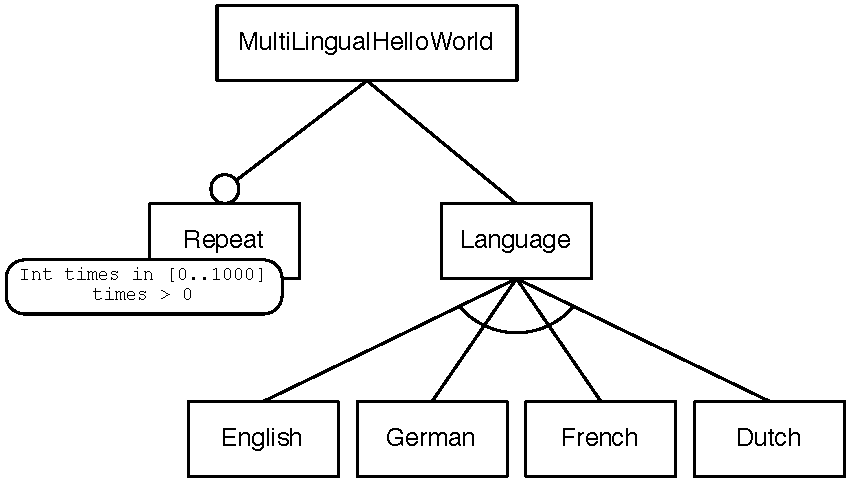
\includegraphics[width=.6\linewidth]{fig/featurediagram}
    \caption{Example feature diagram for a ``Hello World'' software product line}
    \label{fig:feature diagram}
\end{figure}
%
Below we show how the feature model underlying the feature diagram in
Figure~\ref{fig:feature diagram} is encoded in ABS using the textual variability
language \muTVL.
\begin{abscode}
root MultiLingualHelloWorld {
  group allof {
    Language {
      group oneof { English, Dutch, German, French }  
    },
    opt Repeat {
      Int times in [0..1000];
      times > 0; 
    }
  } 
}
extension English {
  Repeat -> (Repeat.times >= 2 && Repeat.times <= 5);
}
\end{abscode}

The ``Hello World'' product line in this example has two main features,
\emph{Language} and \emph{Repeat}, under the root feature and joined with the
\absinline{allof} combinator. The \emph{Language} feature requires one out of
four possible features: \emph{English}, \emph{Dutch}, \emph{French}, or
\emph{German}. The \emph{Repeat} feature is optional, it has no associated
sub-features, and it has an attribute \emph{times} which ranges between 0 and
1000, with an added condition that it must be strictly greater than 0. In this
example an extension for the \emph{English} feature is given. When the
\emph{English} and the \emph{Repeat} features are present, the attribute
\absinline{times} must be between 2 and 5, inclusive.


\subsection{Semantics}

The semantics of \muTVL is given by integer constraints, that is, a feature
model is encoded as a constraint over features and feature attributes. Each
solution for this constraint represents a valid product of the feature model.


\section{Product Selection}
\label{sec:product selection}

ABS allows the developer to name products that are of particular interest, in
order to easily refer to them later when the actual code needs to be generated.
A product definition states which features are to be included in the product and
sets attributes of those features to concrete values.

\subsection{Syntax}
\label{sec:fsl syntax}

Figure~\ref{fig:product selection grammar} shows the grammar of the ABS product selection language. The \NT{Selection}
clause specifies a product by giving it a name, by stating the features and
optional attribute assignments that are included in that product.
% The \NT{FeatureSpec} clause specifies that a given feature is present, and the
% optional \NT{AttributeAssignment} clause is used for specifying the
% attributes, which are assigned concrete values.

% The \NT{InitBlock} clause specifies the
% initialisation block for the given product. This An initialisation block can
% be any core ABS block, but typically will be a simple call to some already
% present \emph{main} method. Initialisation blocks are specified in the product
% selection language to enable product lines with multiple entry points to start
% execution.

\begin{figure}[htp]
    \centering

    \begin{tabular}{rcl}
        \NT{Selection}
        \concrDefn{ \TR{product} \NT{TypeId} \TR{(} \NT{FeatureSpecs} \TR{)} \TR{;} }
        \medskip
        
        \\
        \NT{FeatureSpecs}
        \concrDefn{ \NT{FeatureSpec} \MANYG{\TR{,} \NT{FeatureSpec}} }
        
        \\
        \NT{FeatureSpec}
        \concrDefn{ \fid \OPT{\NT{AttributeAssignments}} }
        \medskip
        
        \\
        \NT{AttributeAssignments}
        \concrDefn{ \TR{\{} \NT{AttributeAssignment} \MANYG{\TR{,} \NT{AttributeAssignment}} \TR{\}} }
        
        \\
        \NT{AttributeAssignment}
        \concrDefn{ \aid \TR{=} \NT{Literal} }
        \medskip
        
        \\      
%       \medskip
        
    \end{tabular}
	\caption{Grammar of the product selection language}
 	\label{fig:product selection grammar}
\end{figure}


\subsection{Example}
A valid product from the example ``Hello World'' product line can be defined as
follows.

\begin{abscode}
product P1 (English);
\end{abscode}
This denotes the inclusion of a single feature, \absinline{English}. Implicitly,
its parent node is also selected. The product \absinline{P2} defined below
includes the features \absinline{Dutch} and \absinline{Repeat}, where
\absinline{Repeat}'s attribute \absinline{times} is initialised to 3. To select
features with attributes, we need to include an assignment of attribute
variables. ABS currently supports boolean and integer feature attributes.
\begin{abscode}
product P2 (Dutch, Repeat{times=3});
\end{abscode}

Below is an \emph{invalid} product definition, that is, one that does not
satisfy the feature model, as the \absinline{Repeat.times} attribute is assigned
a value (2222) outside the valid range defined by the feature model
(\absinline{[0..1000]}). The constraint checker that comes with ABS can evaluate
all product selections with respect to the feature model and warn about invalid
products.
\begin{abscode}
product P3 (English, Repeat{times=2222});
\end{abscode}

\section{Feature Model Reflection}
\label{sec:feat-model-refl}

There is support for limited reflection on the feature model and configured
product in the module \absinline{ABS.Productline}.  The datatype
\absinline{Feature} contains constructors for all feature names.  The function
\absinline{product_features} returns a list of features contained in the
current product, and \absinline{product_name} returns the name of the product,
or the empty string if no product was specified.

The following sample code shows the usage, assuming that product
\absinline{Product} was generated:
\begin{abscode}
module Test;
import * from ABS.Productline;

{
  List<Feature> foo = product_features(); // => Cons(FeatureA, Cons(FeatureC, Nil)) 
  String name = product_name();           // => "Product"
}

productline Test;
features FeatureA, FeatureB, FeatureC;

product Product(FeatureA, FeatureC);
\end{abscode}

% Local Variables:
% TeX-master: "absrefmanual"
% End:
